% Filename: Appendix.tex
% Last update: Monday, 2/13/2019 by Ally Warner
%%%%%%%%%%%%%%%%%%%%%%%%%%%%%%%%%%%%%%%%%%%%%%%%%%%%%%%%%%%%%%%%%%%%%%

\section{ } %No section name for Appendix because the title is given paper_main
\label{sec:Appendix}

The pipeline described in this paper required the use of many software packages and tools. In this appendix, we give more information on how to effectively use these tools specifically for this project and dataset. We have also included images of registration, tensor field creation, simulation, and visualization networks in SCIRun as a preview to the files in the database.

\subsection{DWI Distortion Correction}
\label{sec:distortion}

\subsubsection{FSL Total Readout Time}

Two parameters are frequently required to calculate and apply field maps to correct distortions: the effective echo spacing and the total readout time for an EPI sequence.  We used effective' echo spacing, rather than the actual echo spacing, in order to include the effects of parallel imaging, phase oversampling, etc. We defined effective echo spacing as:
\[
\text{Effective Echo Spacing (s) = 1/(BandwidthPerPixelPhaseEncode * MatrixSizePhase)}
\]

The total readout time (FSL definition) was:
\[
\text{Total readout time (FSL) = (MatrixSizePhase - 1) * EffectiveEchoSpacing}
\]

Total readout time is a necessary input for using FSL's topup and eddy tools for DWI image correction, and can be obtained by using MRIConvert. Details on using MRIConvert are in Section \ref{sec:MRIConvert}.

\subsubsection{MRIConvert}
\label{sec:MRIConvert}

The software package MRIConvert provided acquisition information about the dicom series, as well as converted the MRI to a NiFTI format, including effective echo spacing and total readout time \cite{ref:mriconvert}. 

To obtain this information, we loaded the dicom series for either DWI acquisition. We selected ``Options'' to ensure the DWI was saved in NiFTI format. We then selected ``Convert All'' to save all the files into the output directory specified upon opening MRIConvert. The text file included the FSL-defined total readout time, which was contained in the acquisition parameter file in seconds as a unit. MRIConvert also output the b-values and b-vectors files, which were the same for both the DWI AP and DWI PA scans. The last input file required was an ``index.txt'' file, which contained one column with 65 rows (for 64 directions plus the b0 image) of 1's.

%MRIConvert
\begin{figure}[H]
    \centering
    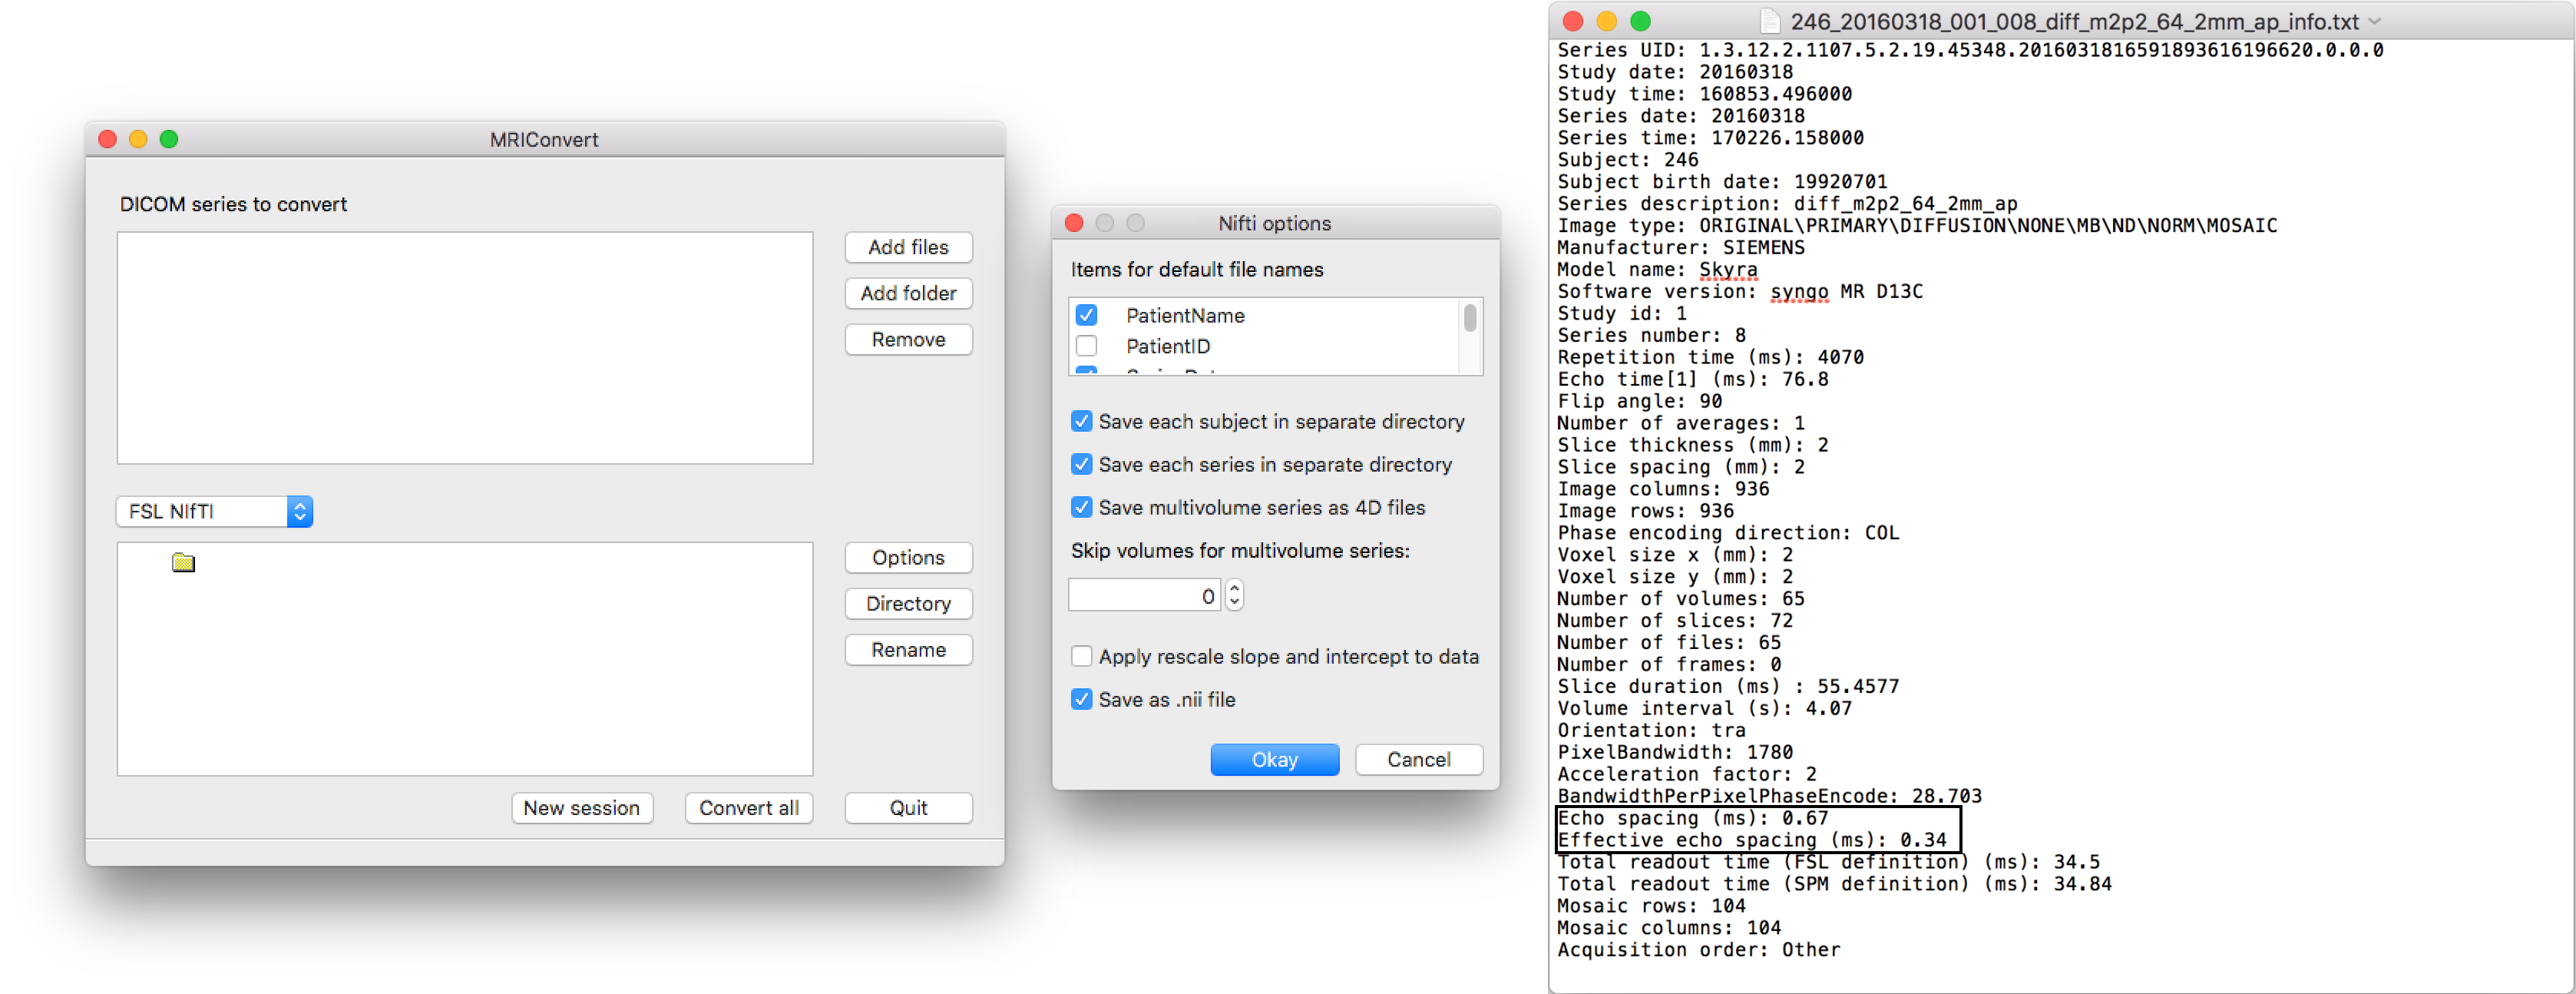
\includegraphics[width=\textwidth]{Figures/combined}
    \caption{MRIConvert \textit{(left)} with options \textit{(middle)} \& output \textit{(right)}.}
    \label{fig:mri_convert}
\end{figure}

\begin{figure}[H]
\centering
{\tt
\begin{varwidth}{\linewidth}
\begin{verbatim}
0  -1 0 0.0345
0   1 0 0.0345
\end{verbatim}
\end{varwidth}
}
\label{fig:acq}
\caption{Acquisition parameters text file.}
\end{figure}

\subsubsection{FSL's Topup and Eddy Command Line Tools}

We made a separate folder for topup results that included the following files: the acquisition parameters file, the index file, b-values, b-vectors, and the DWI AP and DWI PA files. To run topup, we renamed the DWI AP image DWI\_up and the DWI PA image DWI\_down. We renamed the b-values and b-vectors dwi.bval and dwi.bvec, respectively. After all files were in place, we executed the following command line commands:

%topup and eddy command line
\lstdefinestyle{DOS}
{
    backgroundcolor=\color{white},
    basicstyle=\scriptsize\color{black}\ttfamily
}

\begin{lstlisting}[style=DOS]
fslroi DWI\_up b0\_up 0 1
fslroi DWI\_down b0\_down 0 1

fslmerge -t both\_b0 b0\_up b0\_down

topup --imain=both\_b0 --datain=acq_params.txt --config=mine.cnf --out=topup\_results
applytopup --imain=b0\_up,b0\_down --inindex=1,2 --datain=acq_params.txt
           --topup=topup\_results  --out=b0\_hifi

bet b0\_hifi b0\_hifi\_brain -m -f 0.2
eddy --imain=DWI\_up --mask=b0\_hifi\_brain\_mask --index=index.txt --acqp=acq_params.txt
     --bvecs=dwi.bvec --bvals=dwi.bval --fwhm=0 --topup=topup\_results --flm=quadratic
     --out=eddy\_unwarped

\end{lstlisting}

By running these commands, we first obtained the b0 image, which is the baseline image used for calculating field maps for both encoding directions. Then the two b0's were merged together into one file, topup and eddy were applied for distortion correction, and `bet' was applied for brain extraction. The distortion corrected file was named ``eddy\_unwarped.nii.''

\subsection{DTIFIT}
\label{sec:dtifit}

To use DTIFIT we first opened FSL, and then we chose ``FDT Diffusion,'' followed by ``DTIFIT Reconstruct diffusion tensors'' in the drop-down menu, and chose the input files manually; Table \ref{tab:dtifit} lists the files selected.

\begin{table}[H]
\centering
\caption{DTIFIT Input Files}
\label{tab:dtifit}
\begin{tabular}{|c|c|}
\hline
Diffusion weighted data & eddy\_unwarmed.nii        \\ \hline
BET binary brain mask   & b0\_hifi\_brain\_mask.nii \\ \hline
Output basename          & desired output location   \\ \hline
Gradient directions     & dwi.bvec                  \\ \hline
b values                & dwi.bval                  \\ \hline
\end{tabular}
\end{table}

DTIFIT output the eigenvalues (named L1, L2, and L3) and the eigenvectors (named V1, V2, and V3) for the diffusion tensor field. We converted the files from NiFTI format to nrrd format using ITK-SNAP \cite{ref:itksnap}. These are the input files for the SCIRun network in Figure \ref{fig:maketensornet}.

\subsection{NiFTI Toolbox for fMRI Preprocessing}
\label{sec:nifti}

After running the fMRI data through the fcon pipeline, we converted the preprocessed fMRI data from four-dimensional data to two-dimensional data. We opened ``rest.nii'' in Matlab using the ``load\_nii(`rest.nii')'' function within the NiFTI toolbox \cite{ref:nifti}. We then resized the four-dimensional ``img'' variable into a two-dimensional variable for use in SCIRun using Matlab's ``resize" function.

\subsection{EEG Data Matrix in MATLAB}
\label{ref:eegmatlab}

The EEG data was output in an .edf file format. We calculated the EEG signals matrix using a Matlab script called ``edfRead.m.'' \cite{ref:edfread} To run this script, we called ``[hdr, record] = edfread(fname).'' The variable 'record' contained the EEG signals. 

\subsection{Networks}
\label{sec:networks}

\begin{figure}[p]
\begin{center}
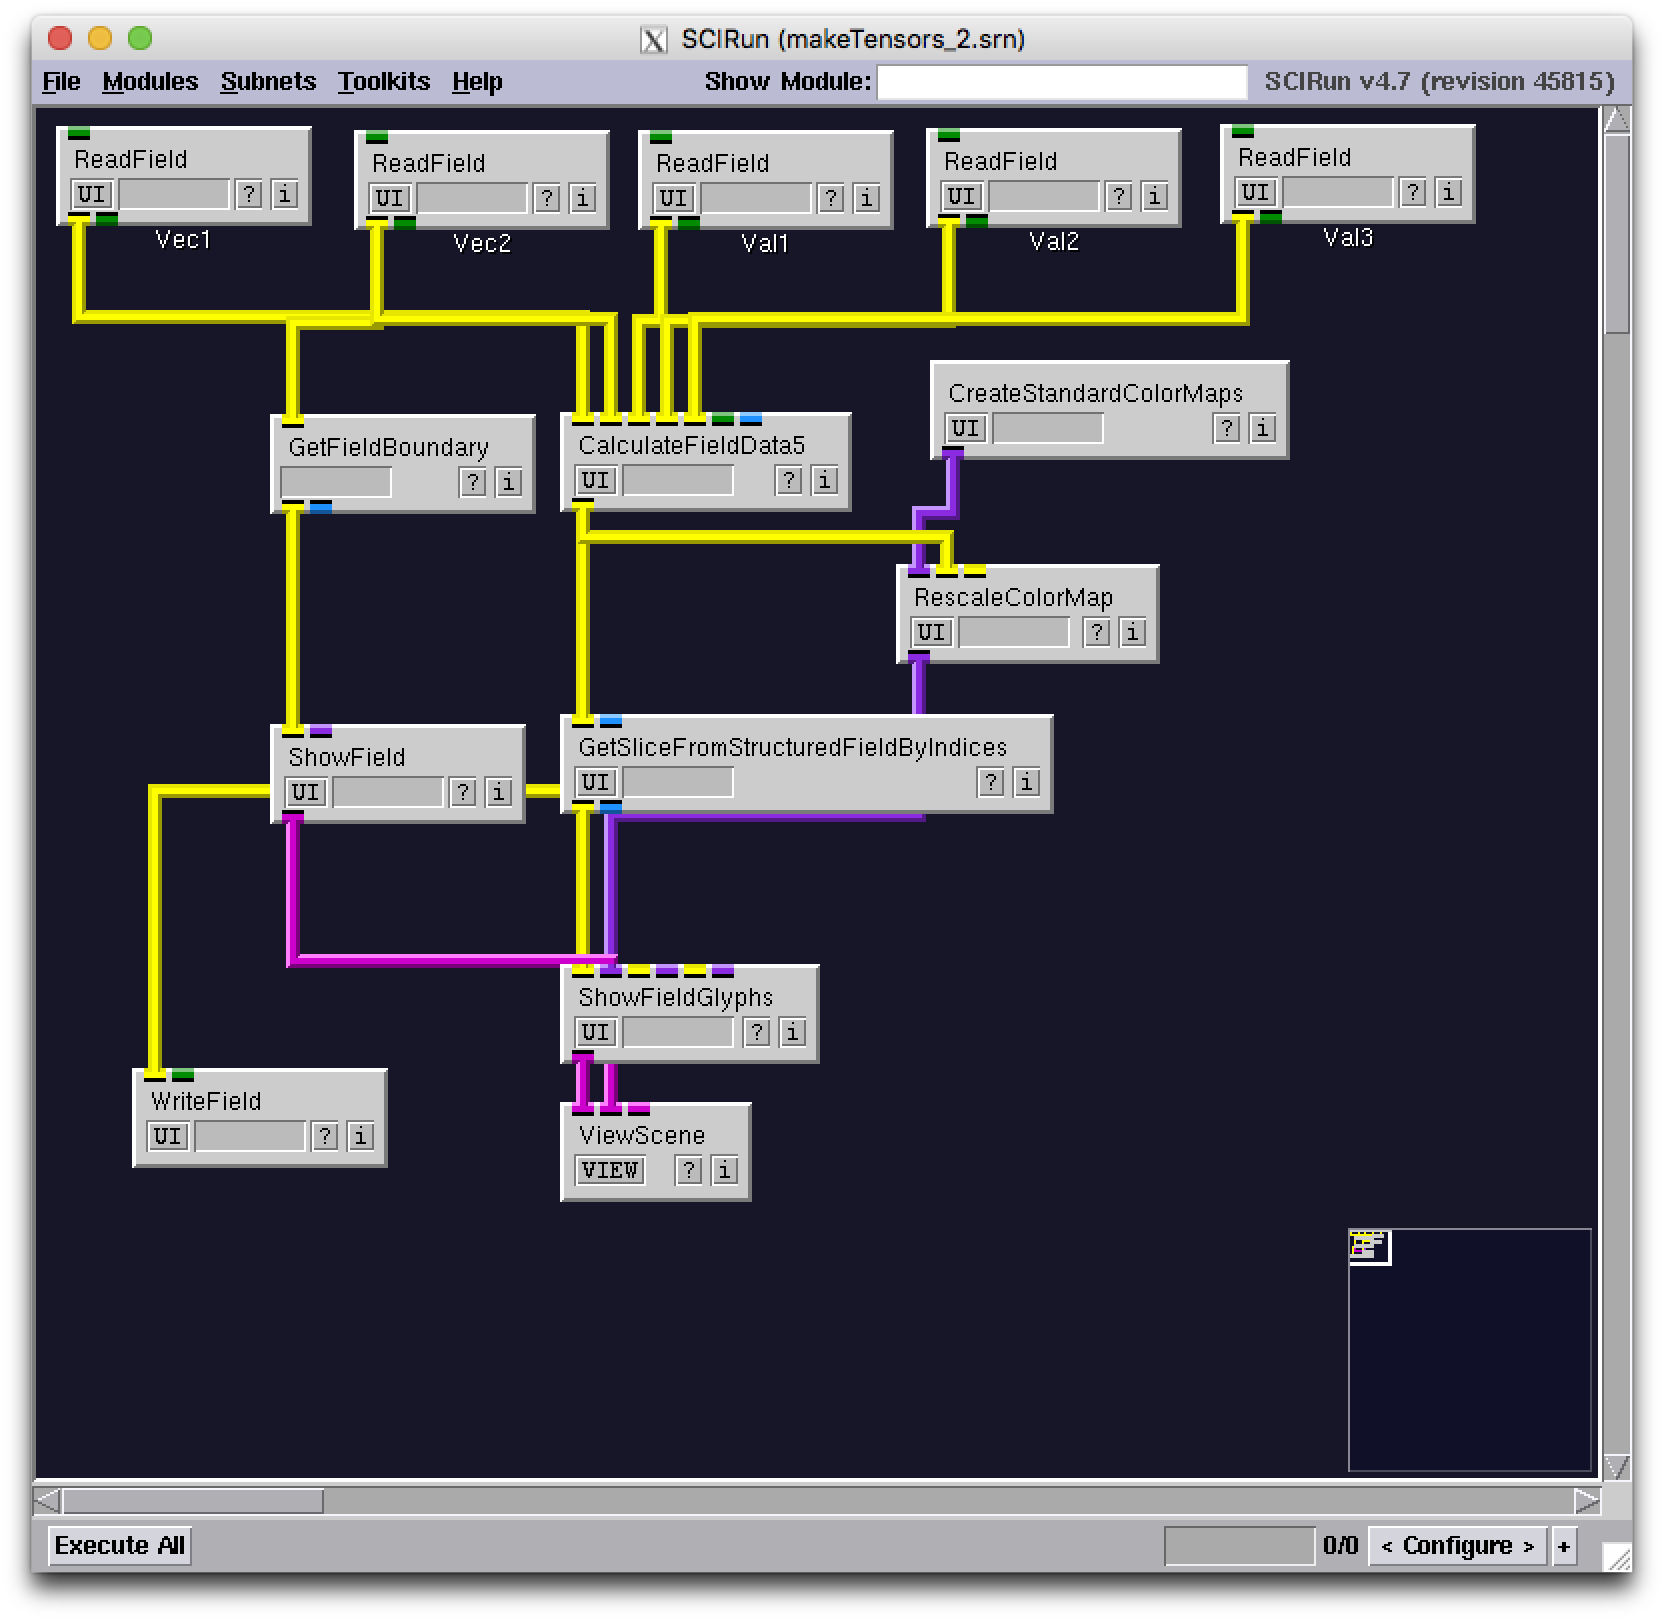
\includegraphics[width=\textwidth]{Figures/make_DTI.png}\\
\caption{SCIRun network to build and visualize diffusion tensor dataset.}
\label{fig:maketensornet}
\end{center}
\end{figure}

\begin{figure}[p]
\begin{center}
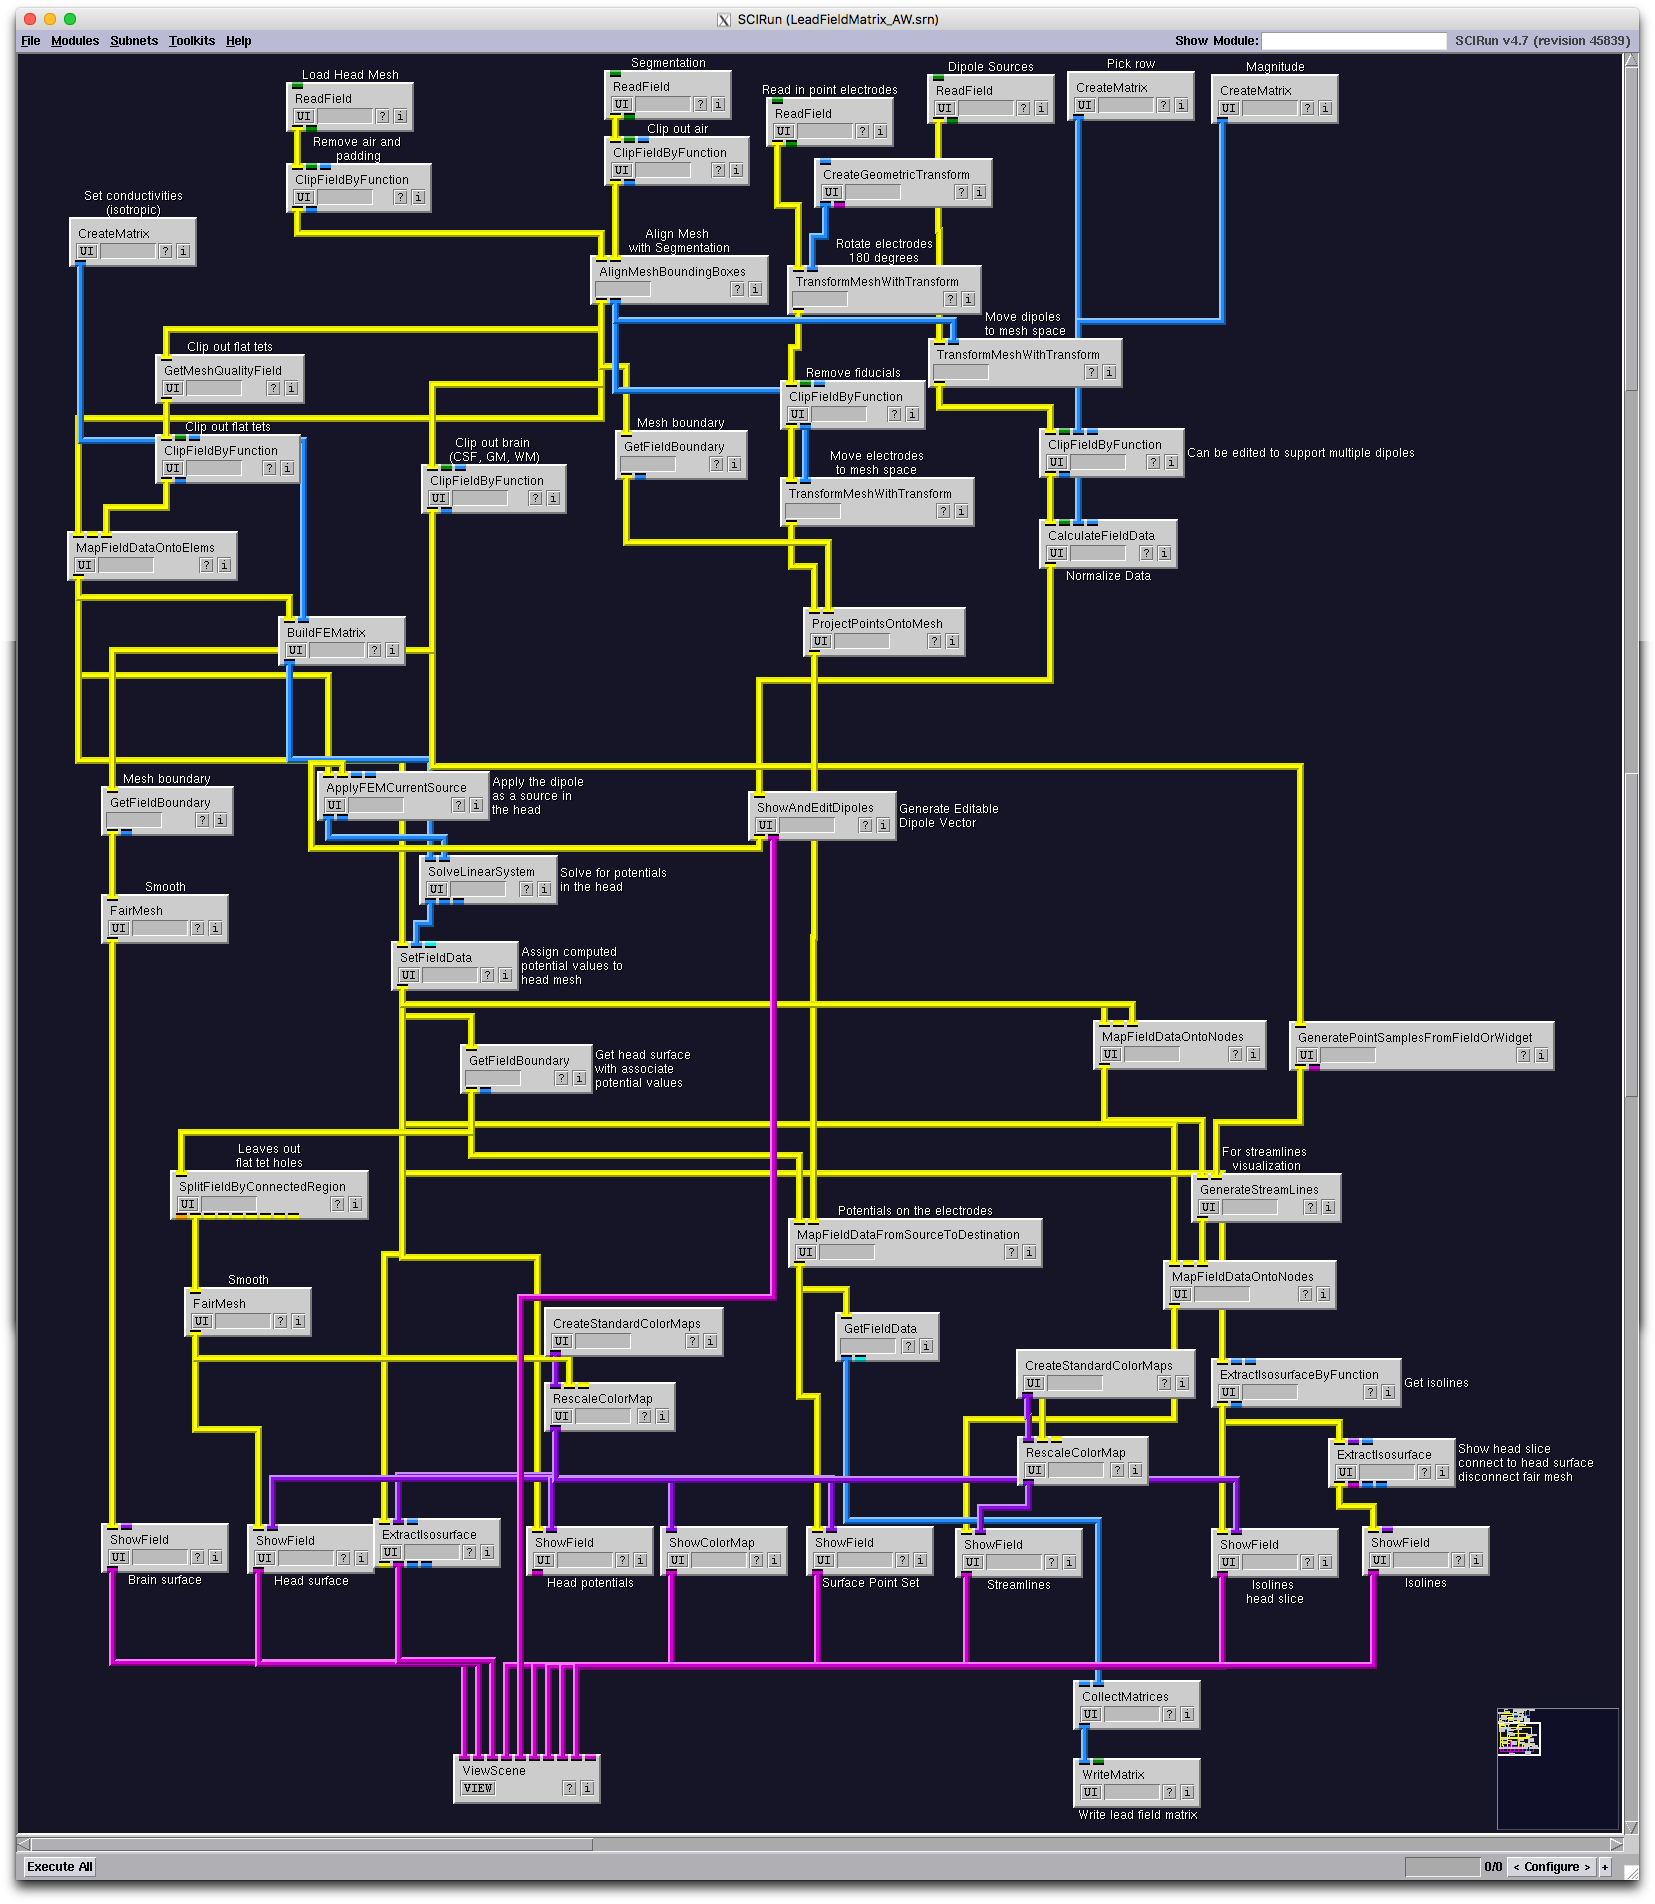
\includegraphics[width=\textwidth]{Figures/iso_network.png}\\
\caption{SCIRun network for isotropic forward problem including registration, visualization, and flat tetrahedra removal.}
\label{fig:isofornet}
\end{center}
\end{figure}

\begin{figure}[p]
\begin{center}
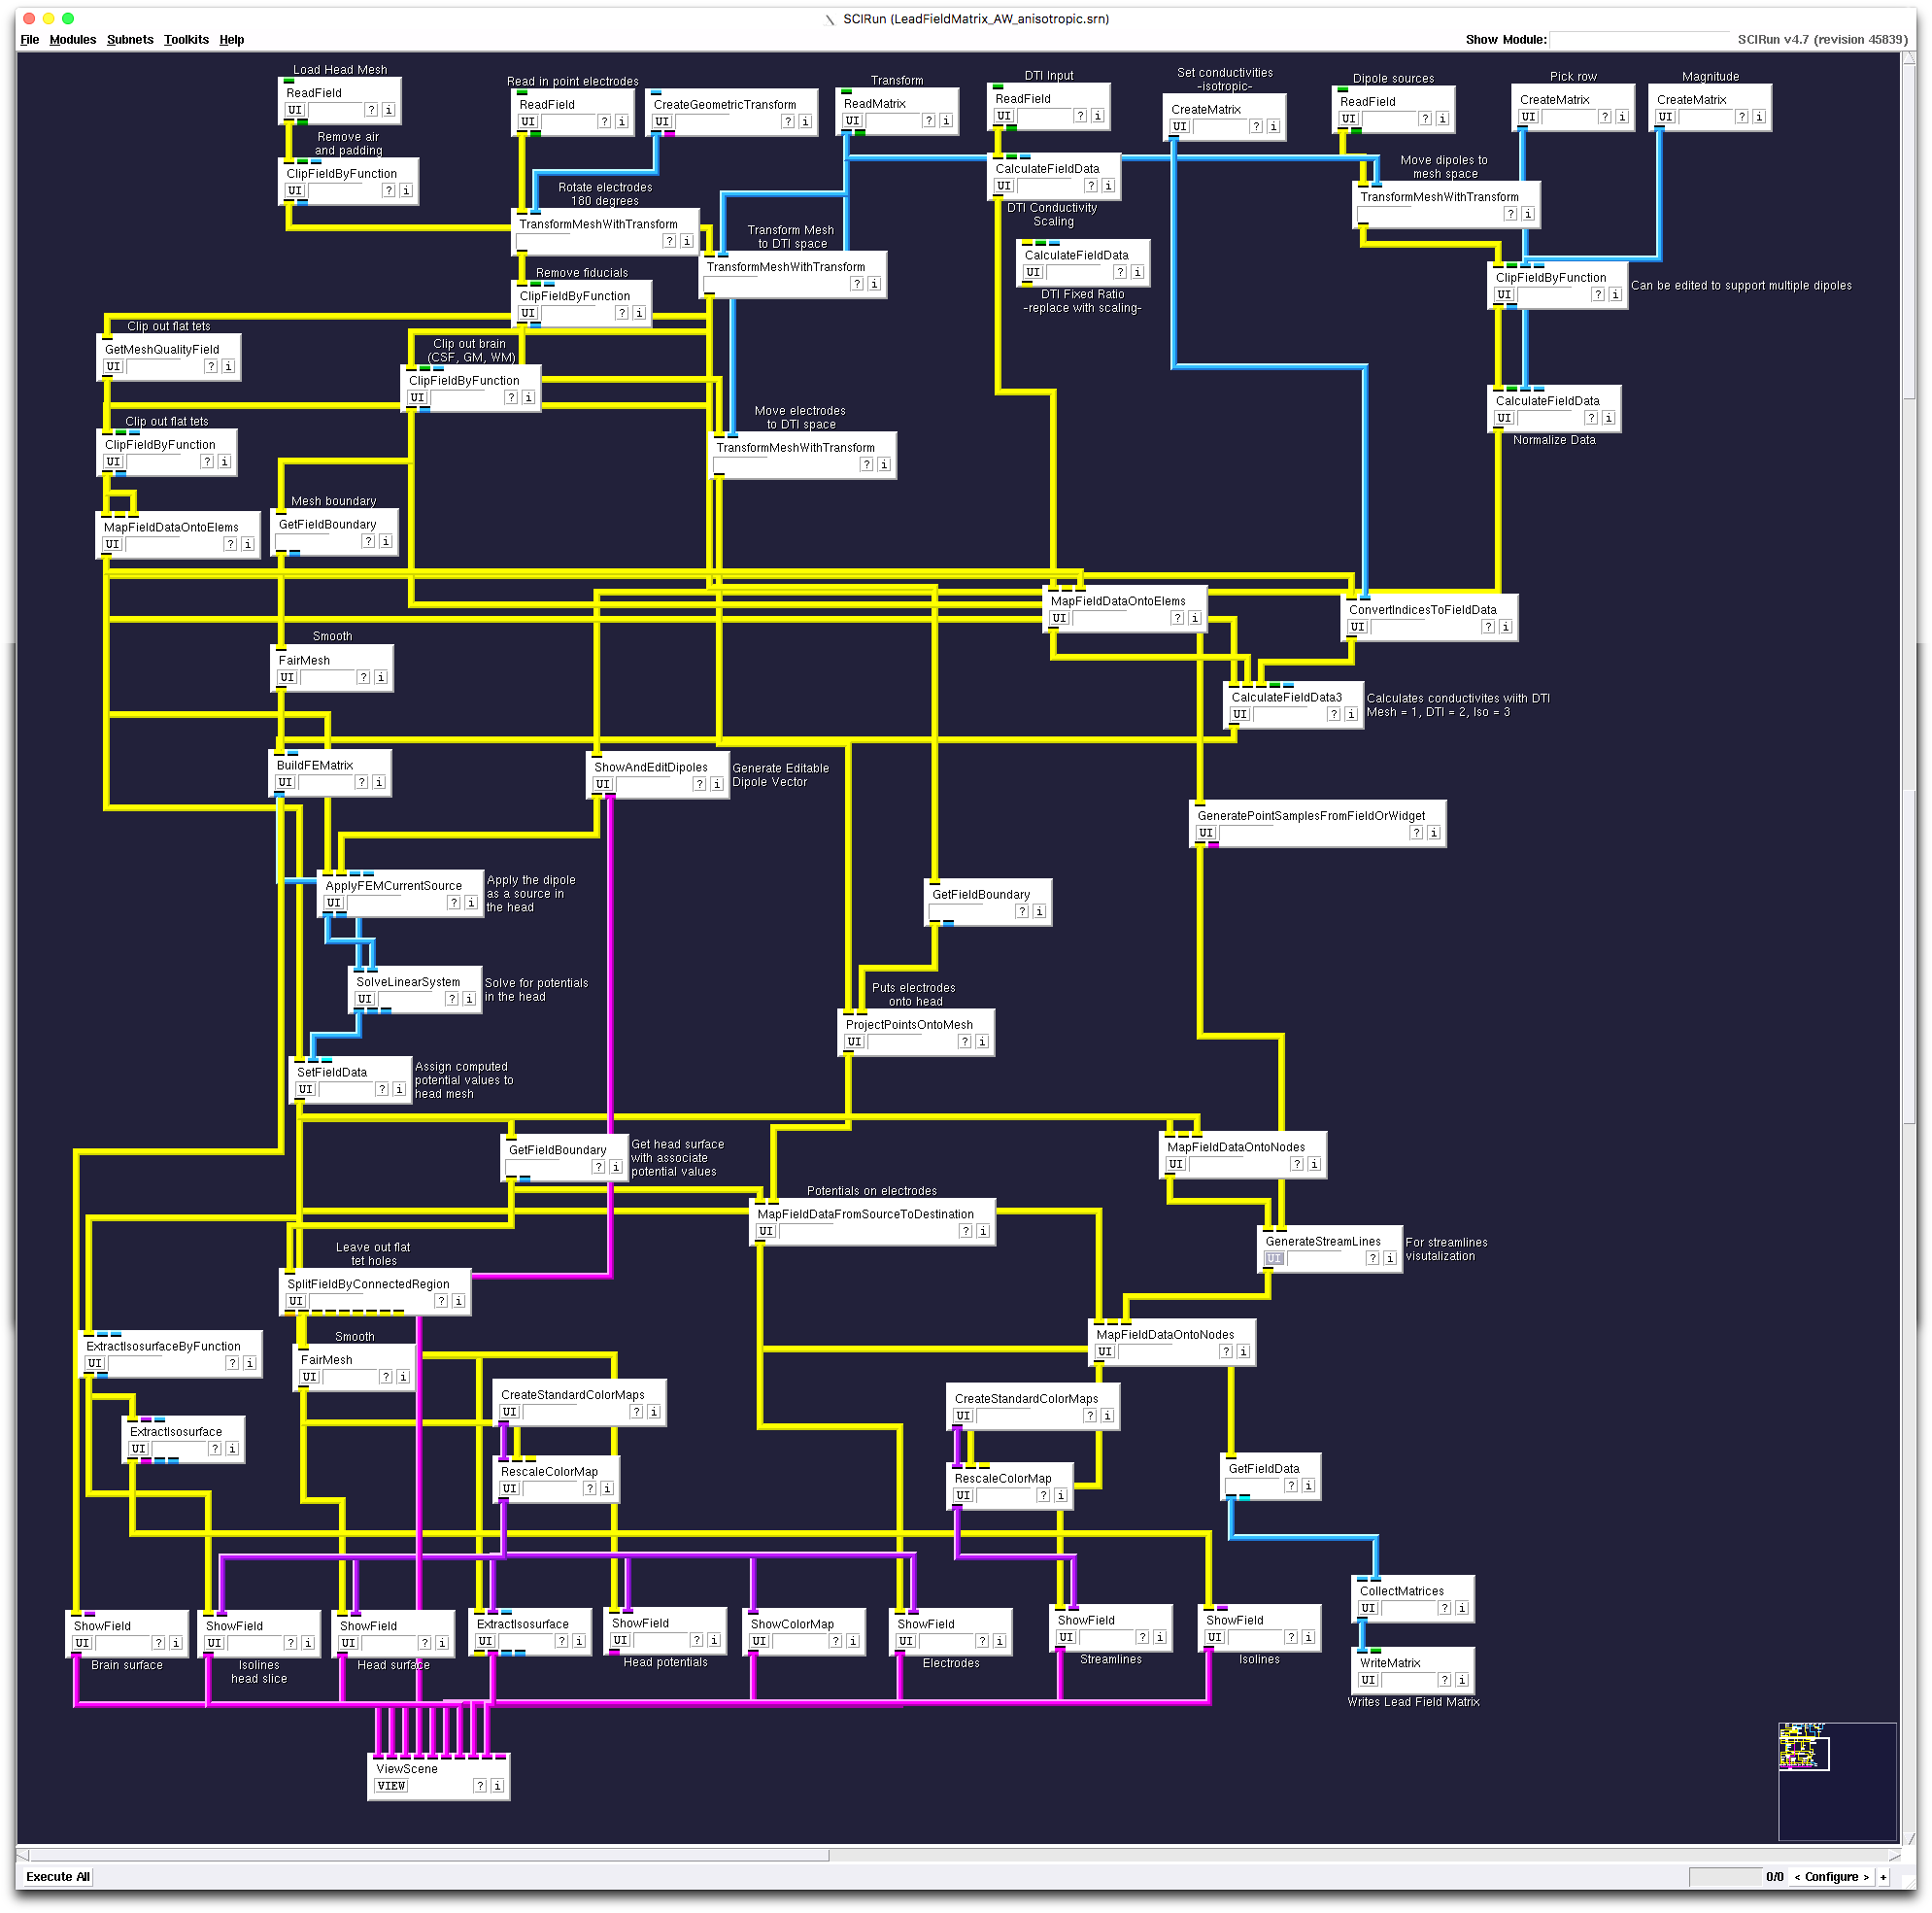
\includegraphics[width=\textwidth]{Figures/aniso_network.png}\\
\caption{SCIRun network for anisotropic forward problem including registration, visualization, and flat tetrahedra removal.}
\label{fig:anisofornet}
\end{center}
\end{figure}

\begin{figure}[p]
\begin{center}
\includegraphics[width=\textwidth]{Figures/fmri_network.png}\\
\caption{SCIRun network for fMRI registration and visualization.}
\label{fig:fmrivisnet}
\end{center}
\end{figure}

\begin{figure}[p]
\begin{center}
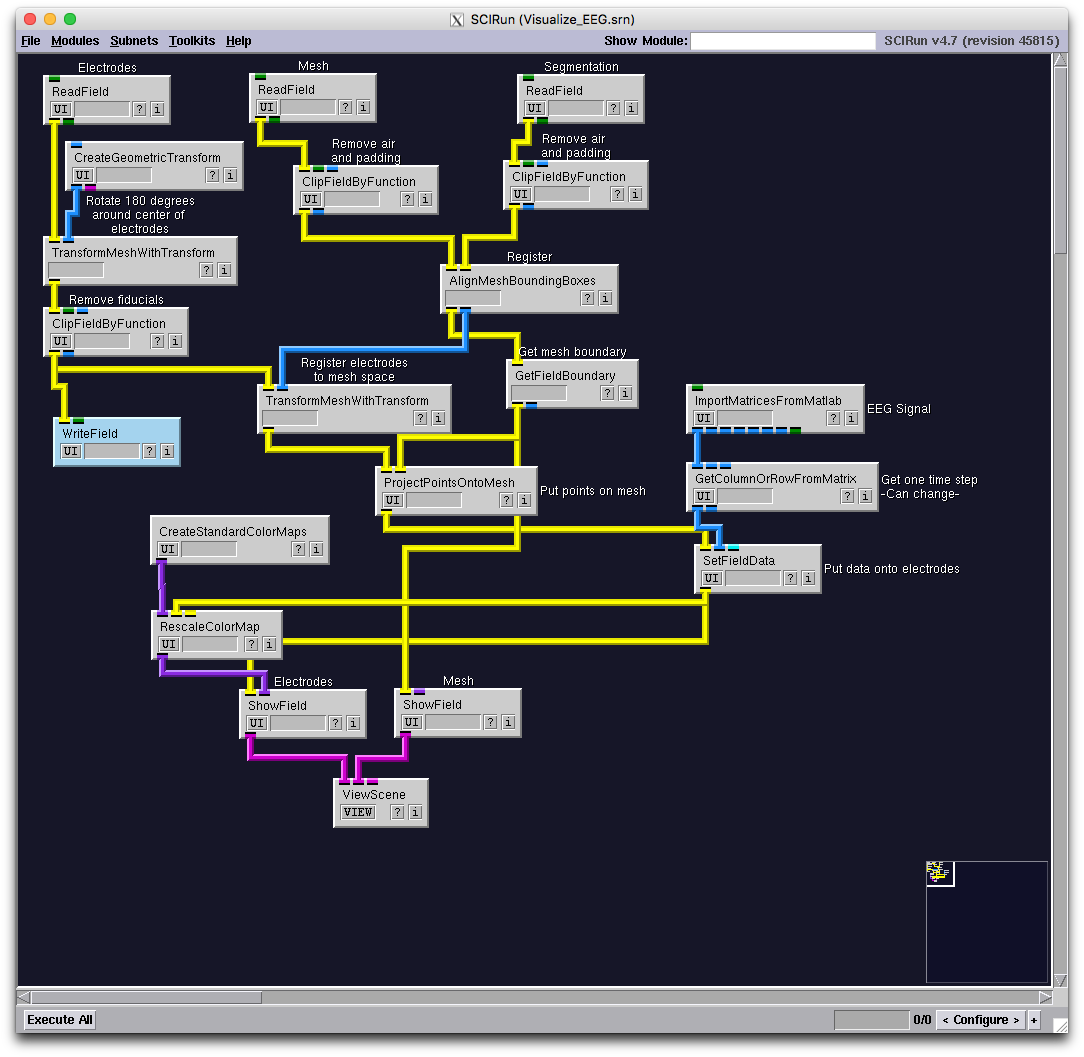
\includegraphics[width=\textwidth]{Figures/EEG_network.png}\\
\caption{SCIRun network for EEG registration and visualization.}
\label{fig:eegvisnet}
\end{center}
\end{figure} 